\maketitle
\tableofcontents
\newpage

\section{Zielsetzung}
Ziel des Versuches ist es, gekoppelte Schwingkreise im Hinblick auf Energietausch
mittels Schwebung und auf ihre Fundamentalschwingungen zu untersuchen.
\section{Theorie}
Die in diesem Versuch gekoppelten Schaltkreise bestehen aus der Induktivität
$L$ und der Kapazität $C$. Die Kopplung besteht aus einem Kopplungskondensator
$C_{\symup{K}}$.
\begin{figure}
  \centering
  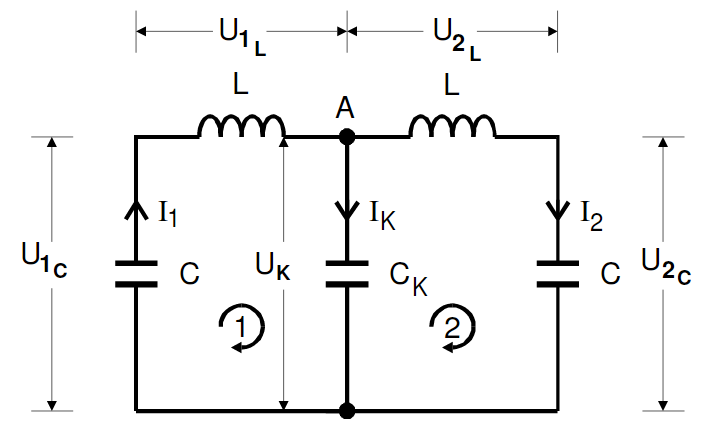
\includegraphics[scale=0.4]{theorie.png}
  \caption{Schaltbild zweier gekoppelter Schwingkreise \cite{anleitung}.}
  \label{fig:1}
\end{figure}
Aus Abbildung \ref{fig:1} lässt sich nun mithilfe der Kirchhoffschen Knoten-
und Maschenregel zwei Schwingungsgleichungen aufstellen
\begin{align}
    L\ddot{I}_1 + \frac{1}{C} \, I_1 + \frac{1}{C_{\symup{K}}} \left(I_1 - I_2\right) &= 0
    \label{eqn:1} \\
    L\ddot{I}_2 + \frac{1}{C} \, I_2 - \frac{1}{C_{\symup{K}}} \left(I_1 - I_2\right) &= 0 \, .
    \label{eqn:2}
\end{align}
Diese Differentialgleichungen sind voneinander abhängig und lassen sich deswegen
nicht ohne weiteres lösen. Durch Subtraktion von \eqref{eqn:1} und \eqref{eqn:2} erhält man
\begin{align}
    L \,  \frac{\symup d^2}{\symup d t^2} \left(I_1 + I_2 \right) + \frac{1}{C} \left(I_1 + I_2 \right) &= 0
    \label{eqn:3} \\
    L \,  \frac{\symup d^2}{\symup d t^2} \left(I_1 - I_2 \right) + \left(\frac{1}{C} + \frac{2}{C_{\symup{K}}} \right)
    \left(I_1 - I_2 \right) &= 0 \, .
    \label{eqn:4}
\end{align}
Damit lassen sich \eqref{eqn:3} und \eqref{eqn:4} unabhängig voneinander lösen; Die
Lösung von \eqref{eqn:3} ist hierbei eine harmonische Schwingung mit der Schwingungsfrequenz
\begin{equation}
    \nu_+ = \frac{1}{2\pi \sqrt{LC}} \, .
     \label{eqn:5}
\end{equation}
Diese Schwingung wird als gleichphasig bezeichnet. Diese wird dadurch ausgezeichnet,
dass beide Schwingkreise so schwingen, als wäre keine Kopplung vorhanden. Wenn man zwei
durch eine Feder gekoppelte Fadenpendel in die gleiche Richtung gleich weit auslenkt,
dann wird die Feder weder gestaucht noch gestreckt, sie verharrt in ihrem unausgelenktem
Zustand. Genauso verhält es sich mit zwei Schwingkreisen, die mit gleicher Amplitude und
Phase anfangen zu oszillieren.

Die Lösung von \eqref{eqn:4} hat die Schwingungsfrequenz
\begin{equation}
  \nu_- = \frac{1}{2\pi \sqrt{L \left(\frac{1}{C} + \frac{2}{C_{\symup{K}}} \right)^{-1}}} \, .
  \label{eqn:6}
\end{equation}
Diese Art der Schwingung wird als gegenphasig bezeichnet. Die Oszillation beginnt
mit gleicher Amplitude, aber entgegengesetzter Phase. Offensichtlich gilt
\begin{equation*}
    \nu_- > \nu_+ \, .
\end{equation*}

\section{Durchführung}
\subsection{Versuchsaufbau}

\subsection{Versuchsdurchführung}

\section{Auswertung}

\section{Diskussion}
\newpage
\nocite{*}
\printbibliography
